\documentclass[tikz,border=2pt]{standalone}
\usepackage{unicode-math}
\setmainfont[
  Path=publication/fonts/,
  UprightFont=source-serif-4-latin-400-normal.ttf,
  ItalicFont=source-serif-4-latin-400-italic.ttf,
  BoldFont=source-serif-4-latin-600-normal.ttf,
  BoldItalicFont=source-serif-4-latin-600-italic.ttf
]{Source Serif 4}
\setmathfont[Path=/System/Library/Fonts/Supplemental/]{STIXTwoMath.otf}
\usepackage{tikz}
\usetikzlibrary{arrows.meta,backgrounds,calc,decorations.pathreplacing,fit,matrix,positioning}
\definecolor{BookInk}{HTML}{18232D}
\definecolor{BookBlue}{HTML}{315F78}
\definecolor{BookRed}{HTML}{98452F}
\definecolor{BookGreen}{HTML}{3F6659}
\definecolor{BookMuted}{HTML}{66727A}
\definecolor{BookRule}{HTML}{AEB7BC}
\tikzset{
  book/node/.style={
    draw=BookInk, line width=.55pt, fill=white,
    minimum height=9mm, inner xsep=5pt, inner ysep=4pt,
    font=\footnotesize, align=center
  },
  book/primary/.style={book/node, draw=BookBlue},
  book/decision/.style={book/node, draw=BookRed},
  book/verified/.style={book/node, draw=BookGreen},
  book/arrow/.style={
    -{Stealth[length=2mm,width=1.35mm]}, line width=.55pt, draw=BookInk
  },
  book/quietarrow/.style={
    -{Stealth[length=2mm,width=1.35mm]}, line width=.45pt, draw=BookRule
  },
  book/feedback/.style={
    -{Stealth[length=2mm,width=1.35mm]}, line width=.5pt,
    draw=BookRed, dashed
  },
  book/note/.style={font=\scriptsize, text=BookMuted, align=center}
}

\begin{document}
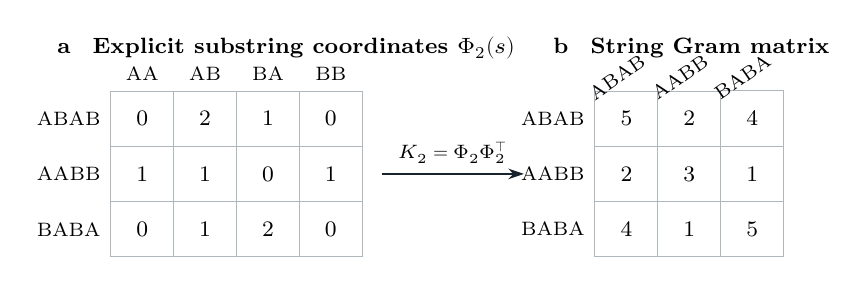
\begin{tikzpicture}
  \node[font=\footnotesize\bfseries,anchor=west] at (0,2.25)
    {a\quad Explicit substring coordinates $\Phi_2(s)$};
  \matrix (phi) [matrix of nodes,nodes={minimum width=8mm,minimum height=7mm,
      draw=BookRule,line width=.35pt,font=\footnotesize},
      row sep=-\pgflinewidth,column sep=-\pgflinewidth] at (2.4,.65) {
    0 & 2 & 1 & 0\\
    1 & 1 & 0 & 1\\
    0 & 1 & 2 & 0\\
  };
  \foreach \j/\lab in {1/AA,2/AB,3/BA,4/BB}
    \node[font=\scriptsize,anchor=south] at (phi-1-\j.north) {\lab};
  \foreach \i/\lab in {1/ABAB,2/AABB,3/BABA}
    \node[font=\scriptsize,anchor=east] at (phi-\i-1.west) {\lab};
  \draw[book/arrow] (4.25,.65)--(6.05,.65)
    node[midway,above,font=\scriptsize] {$K_2=\Phi_2\Phi_2^\top$};
  \node[font=\footnotesize\bfseries,anchor=west] at (6.3,2.25)
    {b\quad String Gram matrix};
  \matrix (gram) [matrix of nodes,nodes={minimum width=8mm,minimum height=7mm,
      draw=BookRule,line width=.35pt,font=\footnotesize},
      row sep=-\pgflinewidth,column sep=-\pgflinewidth] at (8.15,.65) {
    5 & 2 & 4\\
    2 & 3 & 1\\
    4 & 1 & 5\\
  };
  \foreach \j/\lab in {1/ABAB,2/AABB,3/BABA}
    \node[font=\scriptsize,anchor=south,rotate=35] at (gram-1-\j.north) {\lab};
  \foreach \i/\lab in {1/ABAB,2/AABB,3/BABA}
    \node[font=\scriptsize,anchor=east] at (gram-\i-1.west) {\lab};
\end{tikzpicture}
\end{document}
